\documentclass[dvipdfmx]{jarticle}
\usepackage{url}
\usepackage{graphicx}
\usepackage[top=30truemm,bottom=30truemm,left=25truemm,right=25truemm]{geometry}
\title{プログラム設計演習2}
\author{ソフトウェア科学コース\\09B22084山久保孝亮}
\date{\today}

\begin{document}
\maketitle
\section{課題2.4}
\begin{figure}[h]
    \centering
    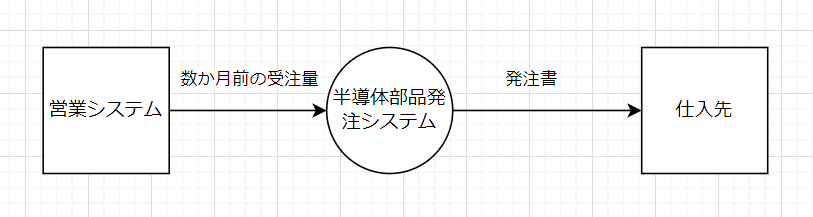
\includegraphics[width=cm]{2-4-1.png}
    \caption{コンテキストダイアグラム}
\end{figure}
\begin{figure}[h]
    \centering
    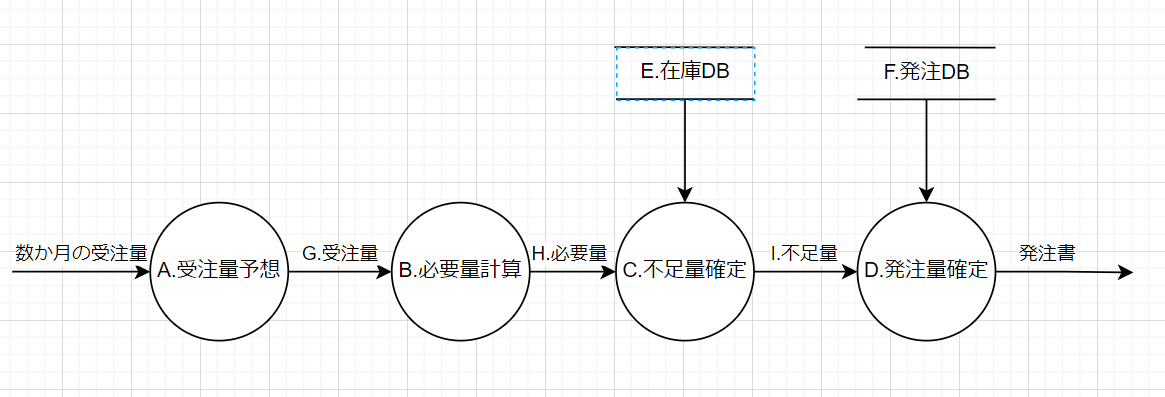
\includegraphics[width=12cm]{2-4-2.png}
    \caption{ダイアグラム0}
\end{figure}
\section{課題2.5}
\begin{figure}[h]
    \centering
    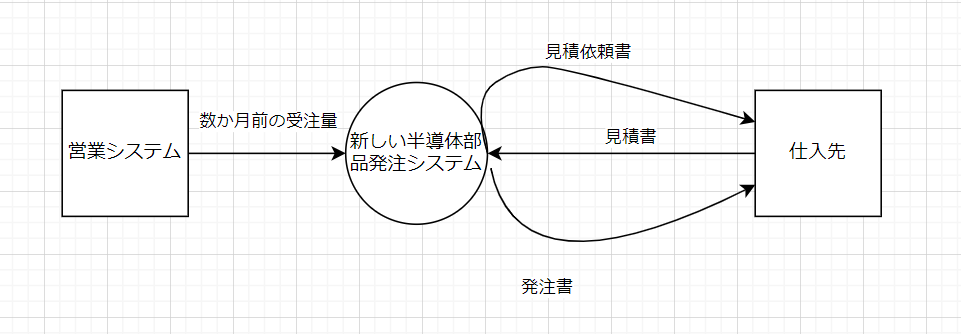
\includegraphics[width=12cm]{2-5-1.png}
    \caption{コンテキストダイアグラム}
\end{figure}
\begin{figure}[h]
    \centering
    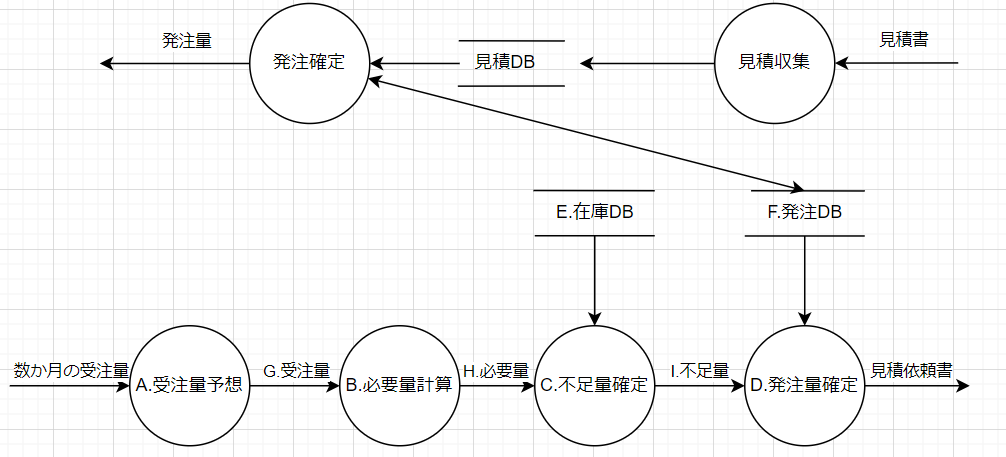
\includegraphics[width=12cm]{2-5-2.png}
    \caption{ダイアグラム0}
\end{figure}
\end{document}